
%(BEGIN_QUESTION)
% Copyright 2011, Tony R. Kuphaldt, released under the Creative Commons Attribution License (v 1.0)
% This means you may do almost anything with this work of mine, so long as you give me proper credit

This single-loop control system has a problem: the pressure indicated on the controller's faceplate shows it to be precisely at setpoint (95 inches W.C.), yet the pressure gauge does not agree. 

$$\includegraphics[width=15.5cm]{i00583x01.eps}$$

Determine the diagnostic value of each of the following tests.  Assume only one fault in the system, including any single component or any single wire/cable/tube connecting components together.  If a proposed test could provide new information to help you identify the location and/or nature of the one fault, mark ``yes.''  Otherwise, if a proposed test would not reveal anything relevant to identifying the fault (already discernible from the measurements and symptoms given so far), mark ``no.''

% No blank lines allowed between lines of an \halign structure!
% I use comments (%) instead, so that TeX doesn't choke.

$$\vbox{\offinterlineskip
\halign{\strut
\vrule \quad\hfil # \ \hfil & 
\vrule \quad\hfil # \ \hfil & 
\vrule \quad\hfil # \ \hfil \vrule \cr
\noalign{\hrule}
%
% First row
{\bf Diagnostic test} & {\bf Yes} & {\bf No} \cr
%
\noalign{\hrule}
%
% Another row
Measure AC line voltage &  &  \cr
%
\noalign{\hrule}
%
% Another row
Measure DC power supply output voltage &  &  \cr
%
\noalign{\hrule}
%
% Another row
Inspect PID tuning parameters in controller &  &  \cr
%
\noalign{\hrule}
%
% Another row
Check pressure transmitter calibration &  &  \cr
%
\noalign{\hrule}
%
% Another row
Measure transmitter current signal &  &  \cr
%
\noalign{\hrule}
%
% Another row
Put controller into manual mode and move valve &  &  \cr
%
\noalign{\hrule}
%
% Another row
Measure DC voltage between TB1-3 and TB1-4 &  &  \cr
%
\noalign{\hrule}
%
% Another row
Measure DC voltage between TB1-7 and TB1-8 &  &  \cr
%
\noalign{\hrule}
} % End of \halign 
}$$ % End of \vbox


\underbar{file i00583}
%(END_QUESTION)





%(BEGIN_ANSWER)

\noindent
{\bf Partial answer:}

% No blank lines allowed between lines of an \halign structure!
% I use comments (%) instead, so that TeX doesn't choke.

$$\vbox{\offinterlineskip
\halign{\strut
\vrule \quad\hfil # \ \hfil & 
\vrule \quad\hfil # \ \hfil & 
\vrule \quad\hfil # \ \hfil \vrule \cr
\noalign{\hrule}
%
% First row
{\bf Diagnostic test} & {\bf Yes} & {\bf No} \cr
%
\noalign{\hrule}
%
% Another row
Measure AC line voltage &  & $\surd$ \cr
%
\noalign{\hrule}
%
% Another row
Measure DC power supply output voltage &  & $\surd$ \cr
%
\noalign{\hrule}
%
% Another row
Inspect PID tuning parameters in controller &  &  \cr
%
\noalign{\hrule}
%
% Another row
Check pressure transmitter calibration &  &  \cr
%
\noalign{\hrule}
%
% Another row
Measure transmitter current signal & $\surd$ &  \cr
%
\noalign{\hrule}
%
% Another row
Put controller into manual mode and move valve &  &  \cr
%
\noalign{\hrule}
%
% Another row
Measure DC voltage between TB1-3 and TB1-4 & $\surd$ &  \cr
%
\noalign{\hrule}
%
% Another row
Measure DC voltage between TB1-7 and TB1-8 &  &  \cr
%
\noalign{\hrule}
} % End of \halign 
}$$ % End of \vbox

Moving the valve in manual mode will be a worthwhile test {\it only} if you also check the gauge's and controller's indications of pressure with the valve in a different position.  Both indications should change with a change in valve position.

%(END_ANSWER)





%(BEGIN_NOTES)

% No blank lines allowed between lines of an \halign structure!
% I use comments (%) instead, so that TeX doesn't choke.

$$\vbox{\offinterlineskip
\halign{\strut
\vrule \quad\hfil # \ \hfil & 
\vrule \quad\hfil # \ \hfil & 
\vrule \quad\hfil # \ \hfil \vrule \cr
\noalign{\hrule}
%
% First row
{\bf Diagnostic test} & {\bf Yes} & {\bf No} \cr
%
\noalign{\hrule}
%
% Another row
Measure AC line voltage &  & $\surd$ \cr
%
\noalign{\hrule}
%
% Another row
Measure DC power supply output voltage &  & $\surd$ \cr
%
\noalign{\hrule}
%
% Another row
Inspect PID tuning parameters in controller &  & $\surd$ \cr
%
\noalign{\hrule}
%
% Another row
Check pressure transmitter calibration & $\surd$ &  \cr
%
\noalign{\hrule}
%
% Another row
Measure transmitter current signal & $\surd$ &  \cr
%
\noalign{\hrule}
%
% Another row
Put controller into manual mode and move valve & $\surd$ &  \cr
%
\noalign{\hrule}
%
% Another row
Measure DC voltage between TB1-3 and TB1-4 & $\surd$ &  \cr
%
\noalign{\hrule}
%
% Another row
Measure DC voltage between TB1-7 and TB1-8 &  & $\surd$ \cr
%
\noalign{\hrule}
} % End of \halign 
}$$ % End of \vbox

The fact that the gauge and controller disagree on pressure tells us the problem is either with the gauge, or with the transmitter-controller signal path.  Nothing else (tuning, power, valve) could cause this to happen.  Therefore, valid tests include anything to help is discern whether there is a problem in the gauge, in the transmitter, in the resistor, or in the controller's PV input.

%INDEX% Troubleshooting review: electric circuit diagnostic test usefulness

%(END_NOTES)


